\chapter{AODV}
\label{chap:aodv}

\vspace{-0.5cm}
\tcolorbox[colback=yellow!20, colframe=yellow!75!black, title=Nota]
La semilla usada durante la práctica es \textbf{2701}
\endtcolorbox
\vspace{1cm}


\section{Ejercicio 1.1}

\subsection{¿Qué nodos reenvían el primer paquete RREQ enviado por static1? ¿Y el segundo RREQ? ¿Por qué?}

El primer paquete RREQ enviado por static1 es procesado y reenviado únicamente por los nodos mobile[10] y mobile [12], a pesar de enviarse con intención de alcanzar todos los nodos de la red (Figura \ref{fig:primer_rreq_reception}). Esto ocurre porque ese primer paquete parte de static1 con un TTL igual a 2. Mobile[10] y mobile[12] son los únicos que se encuentran en un posición dentro del rango de alcance de static1 y que, por tanto, reciben el RREQ con potencia suficiente para intentar procesarlo, reduciéndose el TTL en 1. Después, lo reenvían de forma que, cuando llega a los siguientes nodos, el TTL se reduce 1 más, cayendo a 0 y frenándose el proceso de nuevos reenvíos.

Este comportamiento está justificado en el \href{https://datatracker.ietf.org/doc/html/rfc3561}{RFC 3561 sobre AODV}, que dice que TTL\_START suele ser 1, aunque se recomienda que sea al menos 2 cuando los mensaje se usan para conectividad local. Además, el TTL\_INCREMENT por defecto es 2, por lo que en la siguiente iteración el TTL sería 4.

Debido a lo comentado anteriormente, el segundo RREQ es reenviado por 10 y 12 primero (TTL = 3). Gracias a mobile[10] llega a mobile[3] y mobile[1] (TTL = 2), que lo reenvían de nuevo. Finalmente, mobile[7] y mobile[2] lo reenvían una última vez (TTL = 1). Llegados a este punto, el TTL con el que alcanza los siguientes nodos es 0, por lo que ese segundo RREQ ya no se reenviaría más.

\begin{figure}[H]
    \centering
    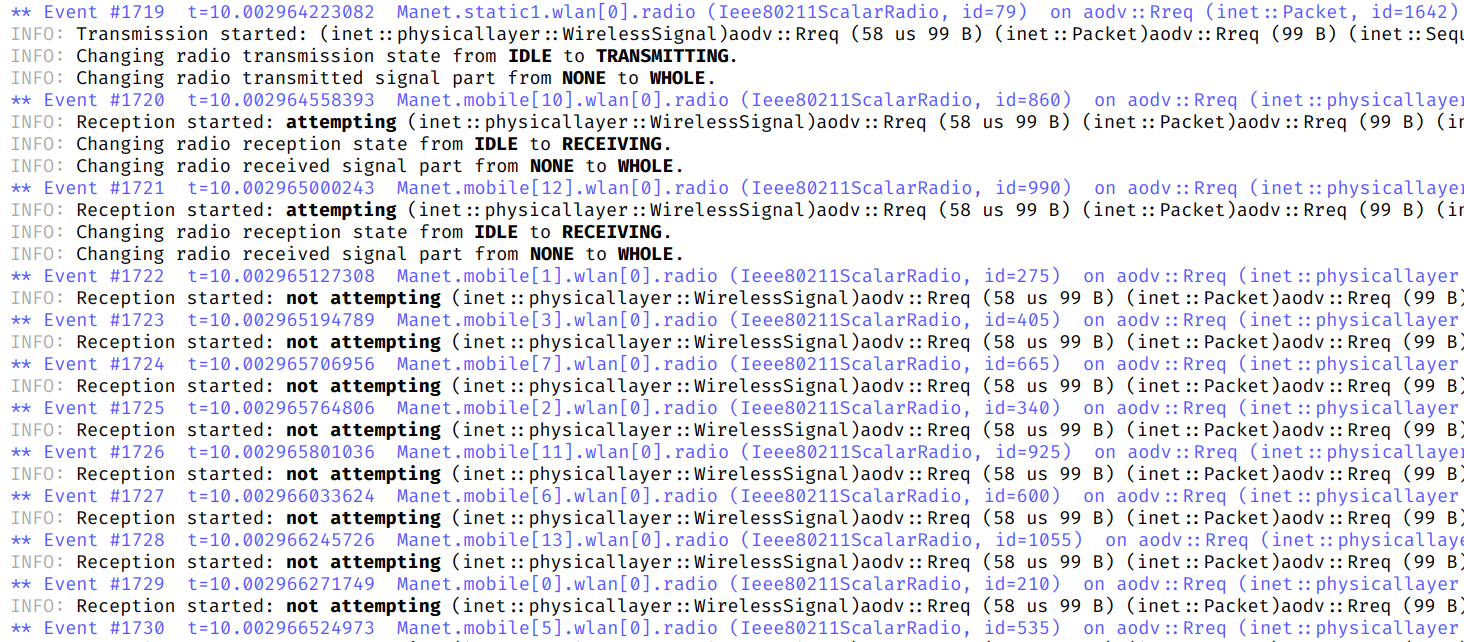
\includegraphics[width=125mm, scale=0.75]{imaxes/ejercicio1_1.png}
    \caption{Logs que muestran el envío del primer RREQ y los nodos que lo reciben}
    \label{fig:primer_rreq_reception}
\end{figure}

\begin{figure}[H]
    \centering
    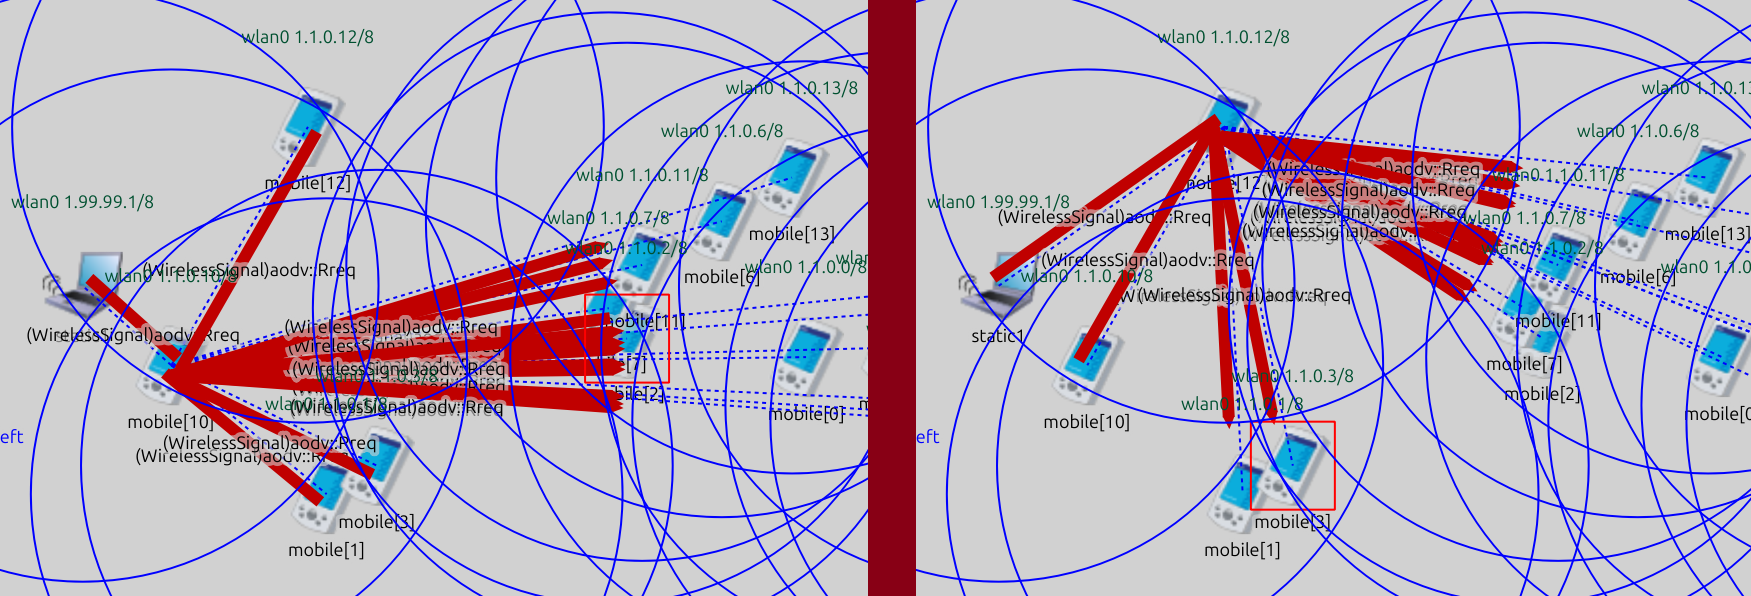
\includegraphics[width=125mm, scale=0.75]{imaxes/ejercicio1_2.png}
    \caption{Nodos que reenvían el primer RREQ (A la izquierda, mobile[10]; A la derecha, mobile[12])}
    \label{fig:primer_rreq_transmission}
\end{figure}

\vspace{1.25cm}
\section{Ejercicio 1.2}

\subsection{Elige el nodo intermedio de la ruta que sigue el primer paquete RREQ que llega a static2. Muestra su tabla
de enrutamiento (vector <Ipv4route *> dentro del módulo ipv4.routingTable) justo antes y justo después de
recibir el primer RREQ. Explica las diferencias y cómo se crean las entradas que aparecen (incluyendo los campos
más importantes).}

Desde el principio de la simulación hasta que llega a mobile[7] el primer RREQ, que es el segundo en términos globales, la tabla de enrutamiento contiene únicamente la dirección del segmento de red, con máscara de subred /8 y /9, y la de localhost (Figura \ref{fig:rtable_prev_mob7}).

Tras recibir el primer RREQ, la tabla de mobile[7] se puebla con dos nuevas entradas (Figura \ref{fig:rtable_post_mob7}). La primera de ellas es la dirección de mobile[3], quien le envía ese primer route request y la segunda es la ruta al origen mediante mobile[3]. Estas rutas nuevas contienen más información en la tabla que las anteriores de acuerdo a las necesidades de AODV. Ambas se generan con la recepción del RREQ y se actualizarán con los RREQ siguientes recibidos por mobile[7]. Vemos como la dirección de destino es la de mobile[3] para una y la de static1 para la otra, mientras que las dos tienen el mismo \textit{gateway} (mobile[3]). Otra diferencia apreciable está en la métrica, que es 3 para el segundo caso debido a que hay tres saltos hasta static1. Finalmente, cabe destacar que ambas tienen el mismo número de secuencia que se incrementa con cada RREQ para indicar que la información esá actualizada, pero la primera entrada se marca como inválida para evitar posibles bucles y mantener solo las rutas necesarias (static1 a través de mobile[3]).

\begin{figure}[H]
    \centering
    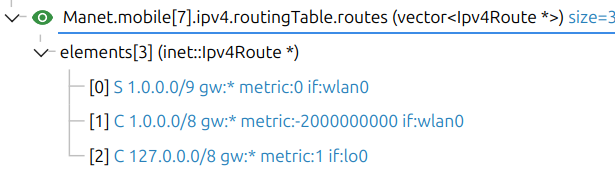
\includegraphics[width=125mm, scale=0.75]{imaxes/ejercicio2_1.png}
    \caption{Tabla de enrutamiento de mobile[7] antes de recibir el primer RREQ}
    \label{fig:rtable_prev_mob7}
\end{figure}

\begin{figure}[H]
    \centering
    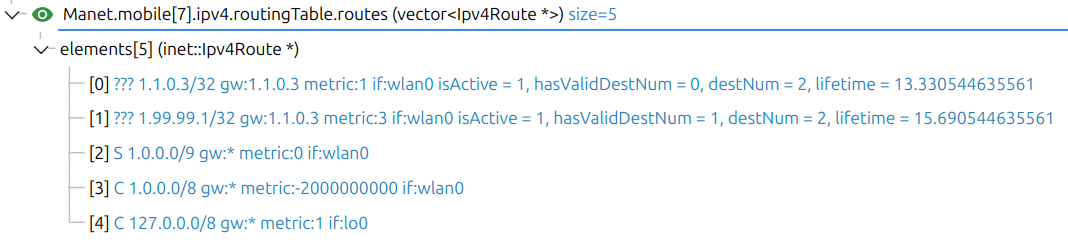
\includegraphics[width=125mm, scale=0.75]{imaxes/ejercicio2_2.png}
    \caption{Tabla de enrutamiento de mobile[7] después de recibir el primer RREQ}
    \label{fig:rtable_post_mob7}
\end{figure}

\vspace{1.25cm}
\section{Ejercicio 1.3}

\subsection{Haz lo mismo justo antes y justo después del primer RREP.}

Como se ve en la figura \ref{fig:rtable_prev_mob7RREP}, antes de que llegue a mobile[7] el primer RREP la tabla de enrutamiento de encuentra mucho más llena que cuando hablábamos del RREQ. Ahora la tabla contiene las direcciones de todos los vecinos directos (Alcanzables en un salto) de mobile[7], además de la ruta a static1.

Por otra parte, la segunda imagen (Figura \ref{fig:rtable_post_mob7RREP}) introduce una entrada más, la de static2. Esta entrada se crea gracias a la recepción del RREP, que intenta rehacer el camino de vuelta al origen desde el destino siguiendo la ruta más corta. Como esta ruta sí es necesaria mantenerla y no es de un vecino de mobile[7], se marca como válida en hasValidDestNum. Podemos ver también que la ruta a mobile[0] y la ruta a static2 tienen un número de secuencia 0. Este número ha sido generado por static2 al enviar el RREP y significa que la ruta es válida y es la de máxima frescura, por lo que es la que será usada para comunicar static1 con static2 (El número de secuencia en AODV es un entero sin signo, por lo que el 0 realmente es el mayor valor representable). Aunque en menor importancia, también podemos fijarnos en que el lifetime de la nueva entrada es mayor que el resto, esto es debido a que se generó más tarde que las otras (Lifetime = Instante actual + ART).

\begin{figure}[H]
    \centering
    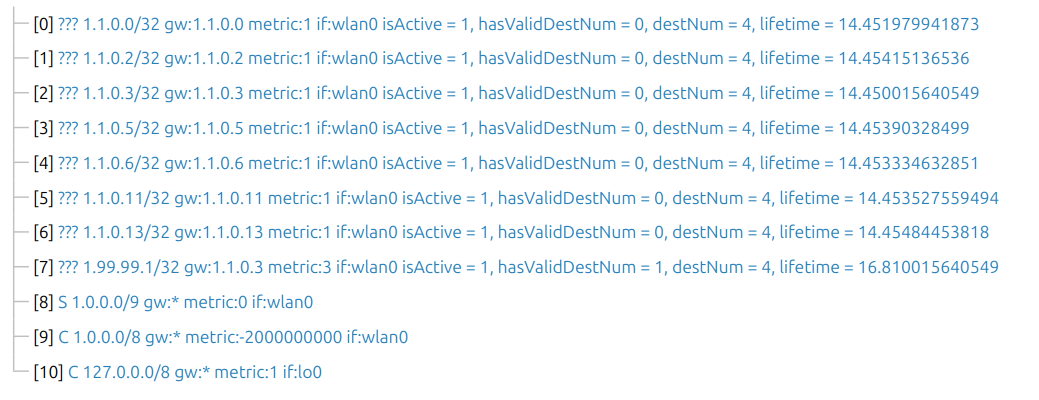
\includegraphics[width=125mm, scale=0.75]{imaxes/ejercicio3_1.png}
    \caption{Tabla de enrutamiento de mobile[7] antes de recibir el primer RREP}
    \label{fig:rtable_prev_mob7RREP}
\end{figure}

\begin{figure}[H]
    \centering
    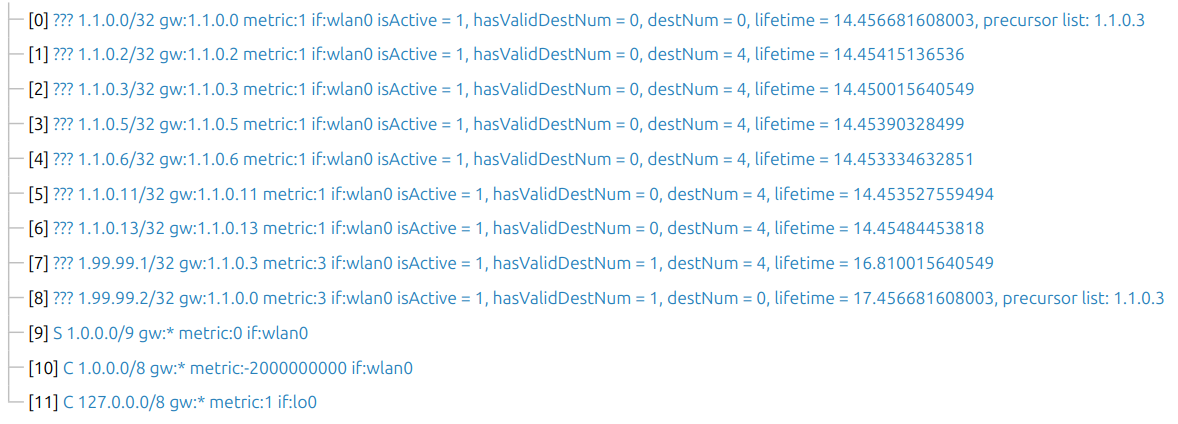
\includegraphics[width=125mm, scale=0.75]{imaxes/ejercicio3_2.png}
    \caption{Tabla de enrutamiento de mobile[7] después de recibir el primer RREP}
    \label{fig:rtable_post_mob7RREP}
\end{figure}

\vspace{1.25cm}
\section{Ejercicio 1.4}

\subsection{Tras aplicar la nueva configuración, ¿Cuál es el primer nodo en darse cuenta de la caída? ¿Cómo? Muestra una captura del log del nodo que se da cuenta que muestre el motivo. ¿Notifica este nodo la caída del nodo?}

Primero de todo, debe aclararse que, como se observa en la figura \ref{fig:escenariot15}, en el escenario producido con la semilla actual, en t=15, los nodos más alejados de static1 que pueden producir una ruta alternativa son mobile[0] y mobile[5], ya que si tirásemos el más cercano a static2 se perdería la comunicación al no haber otro nodo en su rango.

Tras aplicar la configuración para mobile[5] podemos observar en la simulación que este nodo aparece marcado como caído, pero sigue existiendo una ruta hasta static2 (Figura \ref{fig:nodocaidot15}).

Ahora, como vemos en la figura \ref{fig:deteccioncaida}, la caída de mobile[5] es detectada rápidamente por mobile[9], que es el siguiente nodo en el camino hacia static2. Esto ocurre al enviar un paquete UDP de vuelta a static1 desde static2. Mobile[9] intenta contactar durante un período de tiempo con mobile[5], pero al no recibir respuesta, lo marca como ruta inválida.

También podemos ver en los logs (Figura \ref{fig:caidabroadcast}) que mobile[9] notifica a todos los nodos posibles mediante broadcast que mobile[5] no está disponible. En la figura \ref{fig:transmisioncaida} se muestra cómo mobile[9] transmite el paquete RERR y los miembros a su alcance lo reciben (Static2 realiza después el mismo proceso).

\begin{figure}[H]
    \centering
    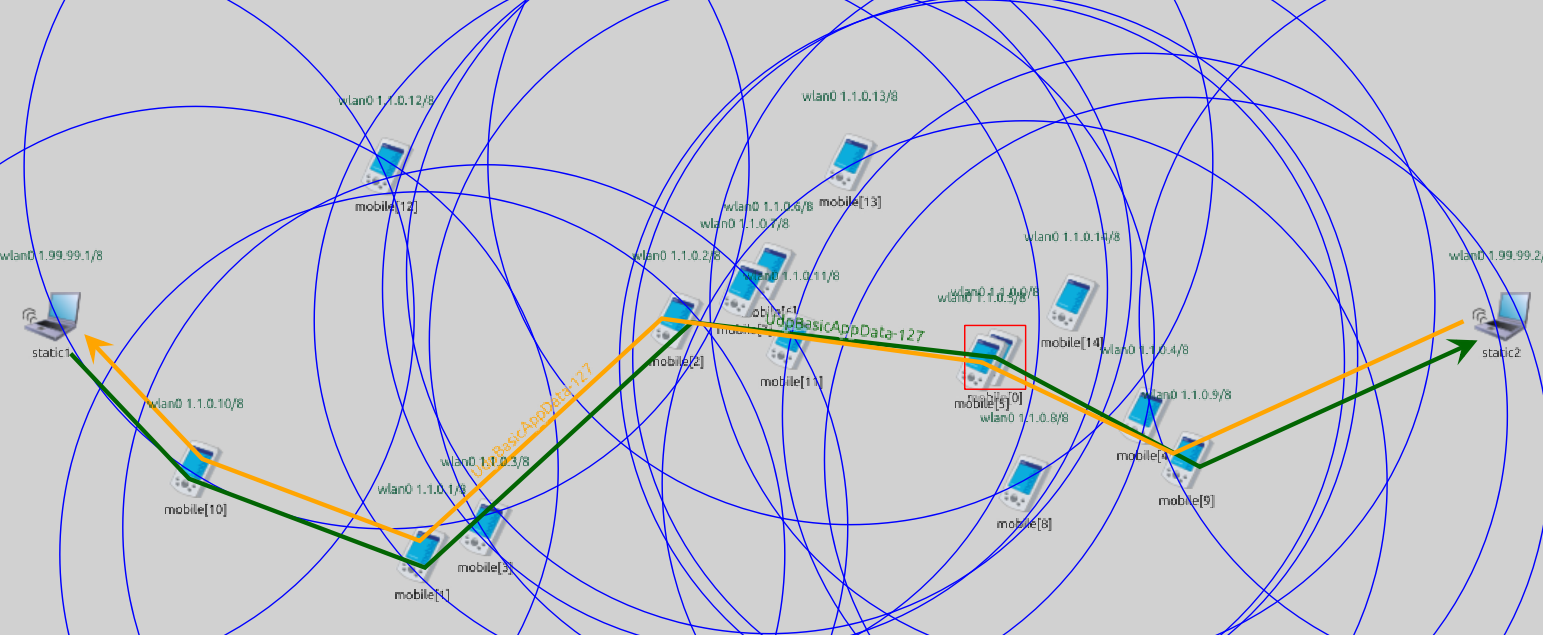
\includegraphics[width=125mm, scale=0.75]{imaxes/ejercicio4_1.png}
    \caption{Escenario en t=15 con todos los nodos en funcionamiento}
    \label{fig:escenariot15}
\end{figure}

\begin{figure}[H]
    \centering
    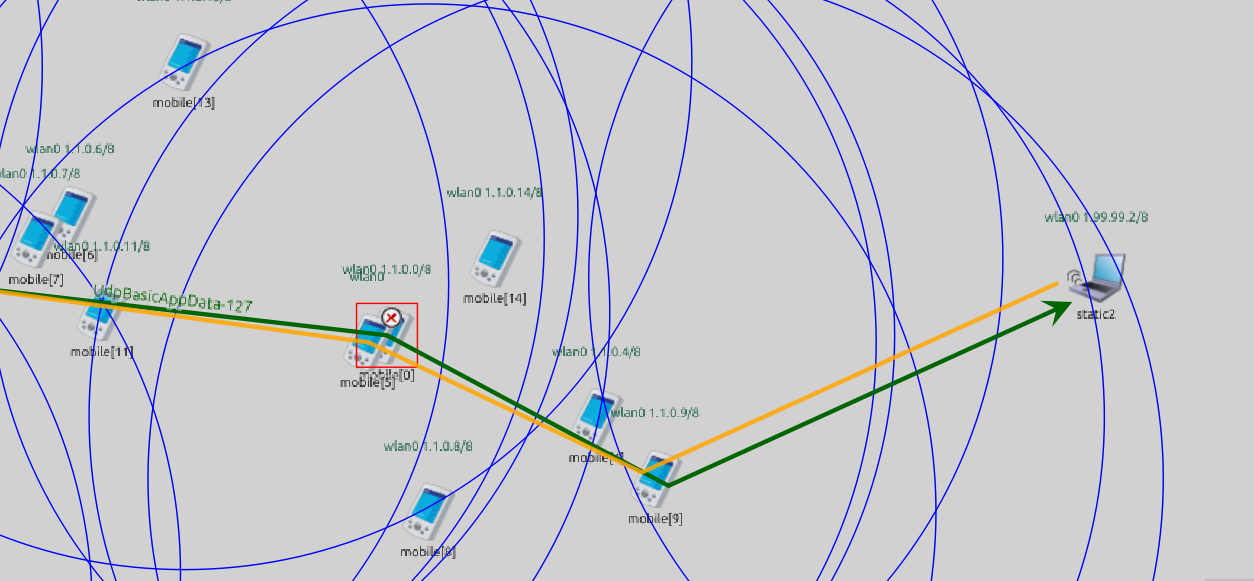
\includegraphics[width=125mm, scale=0.75]{imaxes/ejercicio4_2.png}
    \caption{Detalle de los nodos cercanos a static2 en t=15 con mobile[5] caído}
    \label{fig:nodocaidot15}
\end{figure}

\begin{figure}[H]
    \centering
    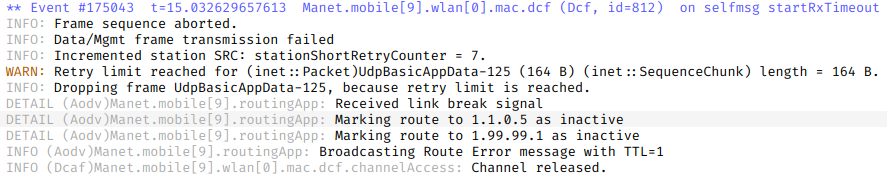
\includegraphics[width=125mm, scale=0.75]{imaxes/ejercicio4_3.png}
    \caption{Log de detección de la caída de mobile[5]}
    \label{fig:deteccioncaida}
\end{figure}

\begin{figure}[H]
    \centering
    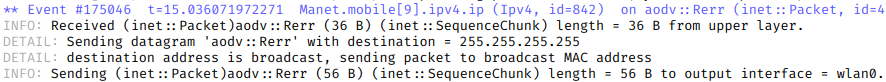
\includegraphics[width=125mm, scale=0.75]{imaxes/ejercicio4_4.png}
    \caption{Log del envío del RRER a broadcast}
    \label{fig:caidabroadcast}
\end{figure}

\begin{figure}[H]
    \centering
    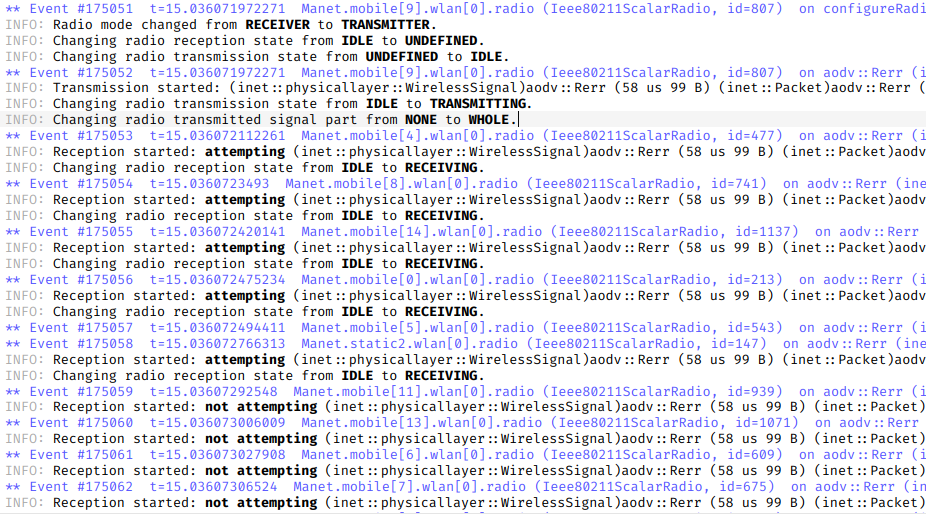
\includegraphics[width=125mm, scale=0.75]{imaxes/ejercicio4_5.png}
    \caption{Logs de la transmisión del RRER por mobile[9]}
    \label{fig:transmisioncaida}
\end{figure}

\vspace{1.25cm}
\section{Ejercicio 1.5}

\subsection{Muestra el contenido del paquete RERR en Wireshark explicando los campos más importantes. ¿Qué IP
tiene como destino? ¿Por qué?}

\section{Ejercicio 1.6}

\subsection{Explica cómo se propaga el RERR por la red. ¿Qué nodos lo reenvían? ¿Cómo sabe un nodo si debe reenviar
el RERR?}

\section{Ejercicio 1.7} 

\subsection{Muestra capturas de la tabla de enrutamiento de un nodo antes y después de recibir un RERR y explica en
qué cambia.}

\section{Ejercicio 1.8}

\subsection{¿Qué hace static1 al recibir el RERR? Muestra el contenido del siguiente RREQ en Wireshark. ¿En qué cambia
con respecto al de la pregunta 1?}